\documentclass[12pt, a4paper]{article}
\usepackage[a4paper, includeheadfoot, mag=1000, left=2cm, right=1.5cm, top=1.5cm, bottom=1.5cm, headsep=0.8cm, footskip=0.8cm]{geometry}
% Fonts
\usepackage{fontspec, unicode-math}
\setmainfont[Ligatures=TeX]{CMU Serif}
\setmonofont{CMU Typewriter Text}
\usepackage[english, russian]{babel}
% Indent first paragraph
\usepackage{indentfirst}
\setlength{\parskip}{5pt}
% Diagrams
\usepackage{graphicx}
\usepackage{float}
% Page headings
\usepackage{fancyhdr}
\pagestyle{fancy}
\renewcommand{\headrulewidth}{0pt}
\setlength{\headheight}{16pt}
%\newfontfamily\namefont[Scale=1.2]{Gloria Hallelujah}
\fancyhead{}

\usepackage{amsmath}

\graphicspath{ {./images/} }

\usepackage{listings}
\lstdefinestyle{lablisting}{
  basicstyle=\scriptsize\ttfamily,
  numbers=left,
  stepnumber=1,
  otherkeywords={EOF, O\_RDONLY, STDIN\_FILENO, STDOUT\_FILENO, STDERR\_FILENO},
  numbersep=10pt,
  showspaces=false,
  showstringspaces=false
}

\newcommand{\specialcell}[2][l]{%
  \begin{tabular}[#1]{@{}l@{}}#2\end{tabular}}

\begin{document}

% Title page
\begin{titlepage}
\begin{center}

\textsc{Федеральное государственное автономное образовательное учреждение высшего\\
образования "Национальный исследовательский университет ИТМО"}
\vfill
\textbf{Лабораторная работа №2\\[4mm]
по дисципение "Информационная безопасность"\\[4mm]
Блочное симметричное шифрование\\[4mm]
}
\textit{Вариант 10\\[20mm]}
\begin{flushright}
Выполнил: студент Саржевский И.А.
\\[2mm]Группа: P3402\\[4mm]
Преподаватель: к.т.н., доцент\\
Маркина Т.А.
\end{flushright}
\vfill
г. Санкт-Петербург\\[2mm]
2021 г.

\end{center}
\end{titlepage}

\begin{huge}Лабораторная работа №2\end{huge}\\[4mm]
\begin{Large}Блочное симметричное шифрование\end{Large}\\

\section*{Цель работы}

Изучение структуры и основных принципов работы современных алгоритмов
блочного симметричного шифрования, приобретение навыков программной
реализации блочных симметричных шифров.

\section*{Задание}

\textbf{Вариант: 4(д)}. Реализовать систему блочного шифрования,
позволяющую шифровать и дешифровать файл на диске с использованием
блочного шифра ГОСТ 28147-89 в режиме шифрования OFB.

Данный блочный шифр реализован на основе итерационной схемы Фейстеля.
Для шифрования необходимо задать один 256-битный ключ, который в
последствии разбивается на 8 32-х битных подключей, которые используются
в 32-х раундах шифрования в определенной последовательности - в первых
23-х раундах подключи циклически повторяются по очереди, и в последнем
проведении подключи выбираются с начиная с последнего. На каждом раунде
шифрования, блок данных складывается с ключом по модулю $2^{32}$, и результат
подается на узлы таблицы замен. Нет четкого требования к алгоритму формирования
этих узлов, было принято решение взять узлы замен определенные 
Техническим комитетом по стандартизации 'Криптографическая защита информации'
Росстандарта. Полученное на выходе число циклически сдвигается на 11 разрядов
вправо.

Режим шифрования OFB предполагает выработку гаммы. Зашифрованный текст получается
применением операции сложения по модулю 2 с блоком открытого текста. Каждая
последующая гамма, использующаяся для шифрования следующего блока данных,
вырабатывается на основании предыдущей используя алгоритм шифрования (в данном
случае ГОСТ 28147-89). При этом, первая гамма вырабатывается на основании
блока данных, задаваемого извне (IV). Расшифровка производится аналогично
шифрованию, при использовании одинакового IV повторное шифрование зашифрованного
текста произведет исходные данные.

Для инициализации работы алгоритма требовались две константы извне - IV для
генерации первой гаммы и 256-битный ключ. Было принято решение, что система
будет принимать файл с секретной фразой, первый 8 байт которой будут считаться
за IV, а следующие 32 байта - за ключ. Таким образом, стороны передачи должны
договориться только об этой секретной фразе. Исходя из назначения, данная
фраза должна иметь длинну не менее 40 байт, это 40 латинских символов в
кодировке UTF8.

\begin{figure}[t]
    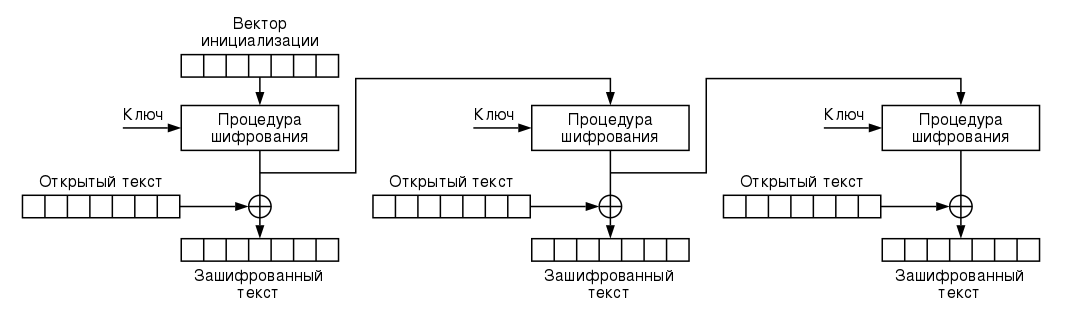
\includegraphics[scale = 0.5]{ofb_enc}
    \caption{Схема шифрования OFB}
    \centering
\end{figure}

\newpage
\section*{Листинг разработанной программы}

\subsubsection*{main.rs}

\lstinputlisting[style=lablisting]{../src/main.rs}

\newpage
\subsubsection*{encrypt.rs}

\lstinputlisting[style=lablisting]{../src/encrypt.rs}

\newpage
\section*{Результаты работы программы}

\begin{figure}[h]
    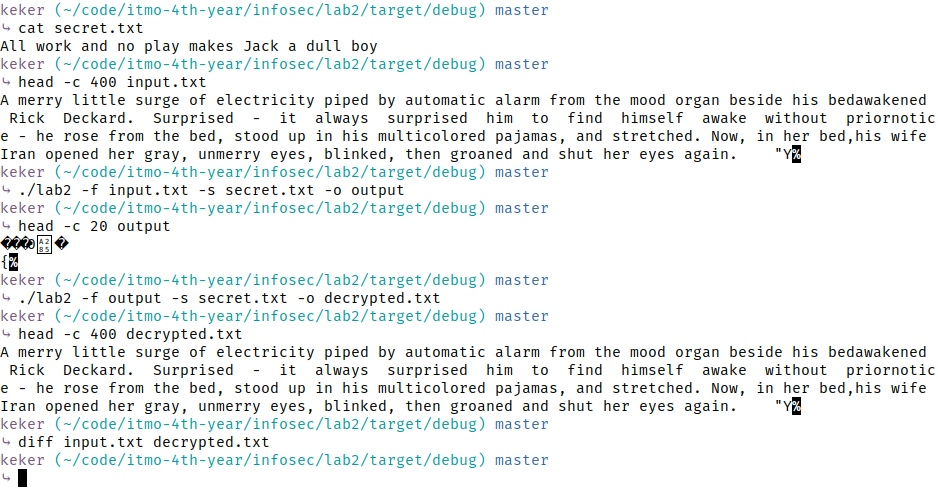
\includegraphics[scale = 0.55]{res}
    \caption{Результат работы программы}
    \centering
\end{figure}

\section*{Вывод}

В ходе выполнения данной лабораторной работы были изучены
принципы работы блочно-симметричных алгоритмов шифрования,
а также разработана программа, имплементирующая шифр
ГОСТ 28147-89 в режиме шифрования OFB.

\end{document}
